\usepackage{tikz}
\usetikzlibrary{arrows.meta, positioning, fit, backgrounds}

\begin{figure}[H]
\centering
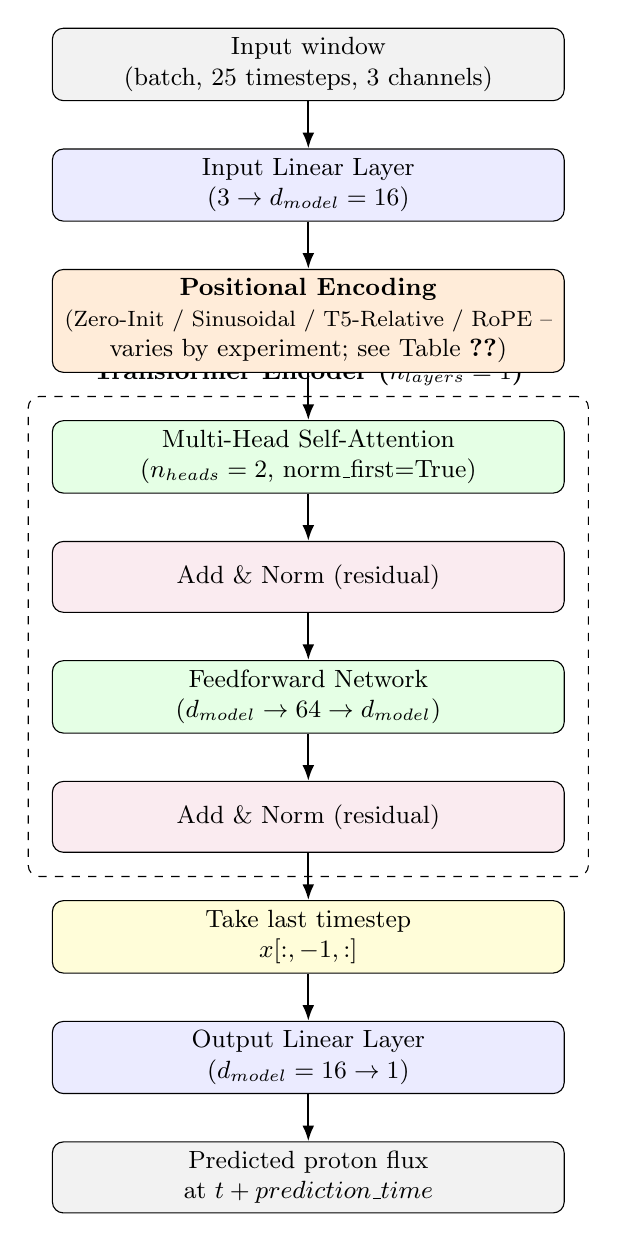
\begin{tikzpicture}[
    node distance=0.6cm,
    box/.style={rectangle, draw, rounded corners, minimum width=6.5cm, minimum height=0.9cm,
                align=center, fill=blue!8, font=\small},
    posbox/.style={box, fill=orange!15},
    encbox/.style={box, fill=green!10},
    poolbox/.style={box, fill=yellow!15},
    arr/.style={-{Latex[length=2mm]}, thick}
]

% Input
\node[box, fill=gray!10] (input) {Input window \\ (batch, 25 timesteps, 3 channels)};

% Input projection
\node[box, below=of input] (proj) {Input Linear Layer \\ ($3 \rightarrow d_{model}=16$)};
\draw[arr] (input) -- (proj);

% Positional encoding (variable component)
\node[posbox, below=of proj] (pos) {\textbf{Positional Encoding} \\ \footnotesize (Zero-Init / Sinusoidal / T5-Relative / RoPE --\\ varies by experiment; see Table~\ref{tab:encoding_comparison})};
\draw[arr] (proj) -- (pos);

% Encoder block
\node[encbox, below=of pos] (attn) {Multi-Head Self-Attention \\ ($n_{heads}=2$, norm\_first=True)};
\draw[arr] (pos) -- (attn);

\node[box, below=of attn, fill=purple!8] (norm1) {Add \& Norm (residual)};
\draw[arr] (attn) -- (norm1);

\node[encbox, below=of norm1] (ff) {Feedforward Network \\ ($d_{model} \rightarrow 64 \rightarrow d_{model}$)};
\draw[arr] (norm1) -- (ff);

\node[box, below=of ff, fill=purple!8] (norm2) {Add \& Norm (residual)};
\draw[arr] (ff) -- (norm2);

% Pooling
\node[poolbox, below=of norm2] (pool) {Take last timestep \\ $x[:, -1, :]$};
\draw[arr] (norm2) -- (pool);

% Output
\node[box, below=of pool] (out) {Output Linear Layer \\ ($d_{model}=16 \rightarrow 1$)};
\draw[arr] (pool) -- (out);

\node[box, below=of out, fill=gray!10] (pred) {Predicted proton flux \\ at $t + \text{prediction\_time}$};
\draw[arr] (out) -- (pred);

% Encoder block bounding box
\begin{scope}[on background layer]
\node[fit=(attn)(norm1)(ff)(norm2), draw, dashed, rounded corners,
      label={[font=\small\bfseries]above:Transformer Encoder ($n_{layers}=1$)},
      inner sep=0.3cm] (encblock) {};
\end{scope}

\end{tikzpicture}
\caption{Encoder-only transformer architecture (M1Transformer). The positional encoding step (highlighted) is the single component varied across the four encoding experiments.}
\label{fig:tikz_architecture}
\end{figure}